% Origen: Secciones/PI - Implementacion Multitrigger.md
\chapter{Implementación -- Multitrigger (MT)}
\label{C:multitrigger}

% Figuras de ESTE capítulo + las compartidas. Siempre al principio del archivo.
\graphicspath{{figs/cap3/}{figs/comunes/}}

\begin{destacado}
En este capítulo describimos el módulo multitrigger: (1) su flujo de utilización
desde el PS, (2) las fuentes de disparo y por qué se combinan con una OR, (3)
las vulnerabilidades de ese mecanismo y cómo se resuelven, y (4) una vista
general del módulo, con el \emph{timestamping} y el tiempo de relanzamiento. Los
detalles de los submódulos, el mapa de registros y la verificación se presentan
en el apéndice, desde la Sec.~\ref{S:ap-mt-submodulos}.
\end{destacado}

Es un módulo secuencial clásico que toma las $N$ \textbf{fuentes de entrada} y
entrega como salida principal los \emph{triggers} de inicio de evento de cada
uno de los $N_s$ \emph{streams} de datos (canales del ADC). En la
Fig.~\ref{f:ap-mt-interfaz} se presentan sus interfaces. Tiene la capacidad
de:
\begin{itemize}
  \item Tener en cuenta hasta $N$ fuentes independientes, en nuestro diseño
    $N=32$.
  \item \textbf{Habilitar las fuentes} con el vector máscara \codigo{OR\_MASK}.
  \item \textbf{Enmascarar eventos}, acción que llamamos escudar
    (\emph{shielding}), con los siguientes parámetros:
  \begin{itemize}
    \item El escudado tiene fuentes, fijadas por \codigo{SHIELD\_SRC}, y
      destinos, fijados por \codigo{SHIELD\_DST}.
    \item Las fuentes de origen (src) de escudado bloquean el disparo de las
      fuentes que reciben el escudo.
    \item La duración es un valor fijo, configurable por registros.
  \end{itemize}
  \item Reportar la última fuente vista mediante un registro interno.
\end{itemize}

Otros detalles importantes de implementación a tener en cuenta:
\begin{itemize}
  \item La condición de funcionamiento estándar es que las \textbf{fuentes
    sean un pulso}, es decir, que duren un ciclo de reloj. \textbf{El disparo
    se considera por nivel alto de la señal de evento}: si una fuente se
    mantuviera alta durante varios ciclos, estaría relanzando la adquisición
    de forma ininterrumpida.
  \item El tiempo de \textbf{relanzamiento del \emph{trigger}}: muchas
    implementaciones de \emph{triggers} no pueden redisparar por una cantidad N de
    ciclos posteriores a un evento. El ejemplo más sencillo es el flanco
    positivo por nivel, en el cual tenemos que partir de la región inferior
    dado un nivel fijo y pasar a una región superior sobre este nivel fijo, de
    forma que no podemos tener dos pulsos seguidos ya que estaríamos partiendo
    de la región superior en el segundo ciclo. Estos valores se exponen mediante registros internos.

\end{itemize}

%%%%%%%%%%%%%%%%%%%%%%%%%%%%%%%%%%%%%%%%%%%%%%%%%%%%%%%%%%%%%%%%%%%%%%%%%%%%%%%%
\section{Flujo de utilización del módulo}
\label{S:mt-flujo}

En la Fig.~\ref{f:mt-secuencia} presentamos esquemáticamente los pasos para
utilizar este módulo:
\begin{enumerate}
  \item \textbf{Desarmado}: escribimos \codigo{OR\_MASK} = 0 en cada canal, para
    que no dispare mientras lo configuramos.
  \item \textbf{Configuración}: escribimos los registros de las fuentes que vamos
    a usar, por ejemplo \codigo{SLOPE\_THR} y \codigo{SLOPE\_HYST} y después
    \codigo{SLOPE\_CFG} con \codigo{en} = 1, y, si hace falta, el escudo en
    \codigo{SHIELD\_CFG}. Fuera de eso, el orden de las escrituras no importa:
    con la máscara en 0 ninguna dispara.
  \item \textbf{\emph{Clear}}: escribimos \codigo{TRIG\_DIS\_CLR}, que borra el
    enganche \codigo{adc\_trg\_dis} y el \codigo{SNAPSHOT} del disparo
    anterior.
  \item \textbf{Armado}: armamos el \emph{scope}, que habilita la escritura al \emph{buffer}
    hasta que llega el disparo y termina el \emph{post-trigger}, y después escribimos
    \codigo{OR\_MASK} con las fuentes de este disparo. Desde ese momento el canal
    dispara con la primera fuente de la máscara.
  \item \textbf{Disparo y lectura}: al disparar, \codigo{mt\_trig\_src} engancha
    \codigo{adc\_trg\_dis}, que bloquea los disparos siguientes del canal. El PS
    sondea \codigo{DIS\_FLAGS} hasta que \codigo{dis\_act} = 1 y lee
    \codigo{SNAPSHOT} para saber qué fuentes dispararon.
  \item \textbf{Re-armado}: para el disparo siguiente volvemos al paso 3, con la
    configuración intacta. En \emph{single-shot} el disparo también borra
    \codigo{OR\_MASK}, por lo que hay que volver a escribirla; en modo continuo
    la máscara persiste y alcanza con el \emph{clear}. El \emph{clear} también lo genera
    \codigo{trigger\_shield} al expirar su \emph{holdoff}, si el canal está entre los
    destinos del escudo.
\end{enumerate}

\begin{figure}[H]
\centering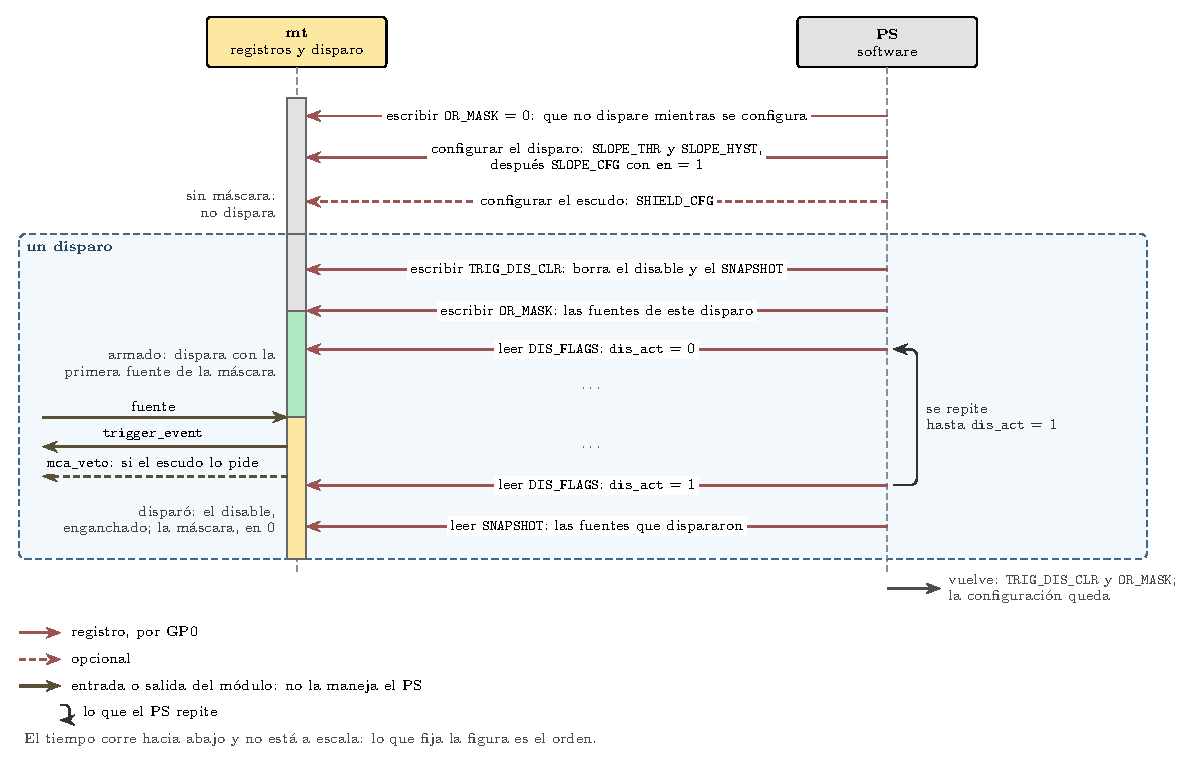
\includegraphics{cap3_mt_secuencia}
\caption[Secuencia de escrituras del PS y respuesta del multitrigger]{%
Secuencia de escrituras y lecturas del PS y respuesta del
multitrigger.\label{f:mt-secuencia}}
\end{figure}

%%%%%%%%%%%%%%%%%%%%%%%%%%%%%%%%%%%%%%%%%%%%%%%%%%%%%%%%%%%%%%%%%%%%%%%%%%%%%%%%
\section{Fuentes de \emph{triggering}}
\label{S:mt-fuentes}

La cantidad de \emph{triggers} disponibles en el módulo es parametrizable. El
diseño original contaba con $N_t=16$; como queríamos agregar fuentes con nuevos
tipos de eventos (nuestra primera idea fue agregar \emph{triggers} por pendiente), decidimos doblar la
cantidad a $N_t=32$. Podríamos tomar un número mayor, pero por un lado no lo
vimos necesario, porque no creemos que haga falta usar simultáneamente tantas
fuentes independientes, y por otro lado aumentar la cantidad requiere más
recursos y complejiza el \textbf{\emph{timing}}.

Los \emph{triggers} presentes en el diseño original consistían en los siguientes:
\begin{itemize}
  \item \textbf{ADC por nivel}: podemos decidir los que queramos, en un primer
    momento ponemos 4 dependiendo del modelo Red Pitaya (n/p).
  \item \textbf{ASG}: \emph{trigger} de la generación de señales interna (n/p).
  \item \textbf{\emph{External}}: \emph{triggers} externos (n/p).
  \item \textbf{Manual}: un \emph{trigger} manual.
\end{itemize}

%%%%%%%%%%%%%%%%%%%%%%%%%%%%%%%%%%%%%%%%%%%%%%%%%%%%%%%%%%%%%%%%%%%%%%%%%%%%%%%%
\section{Elección de fuentes}
\label{S:mt-eleccion}

Cada \emph{stream} de captura $i \in \{1,\ldots,N_\text{CH}\}$ decide el inicio de un
evento a partir de las mismas $N$ fuentes de disparo. Se instancia un
\codigo{mt\_trig\_src} por \emph{stream} de datos, y cada uno combina las fuentes en una única
señal de disparo. La pregunta de diseño es qué función de disparo
$f(\text{trig}_1,\ldots,\text{trig}_N)$ implementar.

En un primer momento parecería que la lógica combinacional es una buena idea.
Partimos de $f(\vec 0)=0$, es decir, si no tenemos ninguna fuente no queremos
un disparo de evento. Analizamos el caso más sencillo, dos entradas
($\text{trig}_1, \text{trig}_2$), para las que tenemos las siguientes
opciones:
\begin{itemize}
  \item OR($\text{trig}_1, \text{trig}_2$): independiente.
  \item AND($\text{trig}_1, \text{trig}_2$): coincidencia~\cite{Knoll2010,Rossi1930}.
  \item XOR($\text{trig}_1, \text{trig}_2$): anticoincidencia (veto)~\cite{Leo1994}.
\end{itemize}

La implementación combinacional tiene dos detalles:
\begin{enumerate}
  \item \textbf{Configuración exponencial.} Especificar $f$ arbitraria requiere
    su tabla de verdad, $2^N$ bits. El espacio de funciones con $f(\vec 0)=0$
    tiene $2^{2^N-1}$ elementos. Y aun para $N$ chico, obliga al usuario a
    enumerar todas las n-tuplas, lo que no es deseable.
  \item \textbf{Trabajo sobre el mismo ciclo de \emph{clock}.}
  \begin{enumerate}
    \item Una función combinacional compara las fuentes \textbf{en el mismo ciclo
      de reloj}. Distintos tipos de fuentes originarias de un mismo pulso
      (nivel, pendiente, externa) llegan con retardos relativos distintos y en
      general dependientes de la amplitud.
    \item Y en el caso de la entrada externa se suman la propagación y la
      sincronización entre dominios de reloj. Las latencias internas se pueden
      compensar en hardware, pero estas no. Una AND o una XOR de un solo ciclo
      es, entonces, frágil: su resultado depende del desfase entre fuentes y no
      sólo de qué fuentes se activaron.
  \end{enumerate}
\end{enumerate}

De las tres funciones vistas, la OR es la única que asegura la adquisición
independientemente del alineamiento de las fuentes en la entrada; esto quiere
decir que \textbf{al menos tenemos un \emph{trigger} por pulso} y como mucho
disparamos datos de más.
Para la AND y la XOR eso exige que los disparos coincidan exactamente, lo que en
la práctica no ocurre, y podemos obtener este análisis en un futuro mediante la
adquisición total y el procesamiento \emph{offline}.

%%%%%%%%%%%%%%%%%%%%%%%%%%%%%%%%%%%%%%%%%%%%%%%%%%%%%%%%%%%%%%%%%%%%%%%%%%%%%%%%
\section{Vulnerabilidades del mecanismo por OR}
\label{S:mt-vulnerabilidades}

El costo de la OR es que un \textbf{mismo pulso puede activar varias fuentes}, y una \textbf{OR sola lo
contaría como varios eventos}. Eso se resuelve con una
ventana de duración $W$ iniciada por el primer disparo. Durante esa ventana, los
disparos siguientes se consideran parte del mismo evento. En el diseño la
ventana se implementa en dos niveles:
\begin{itemize}
  \item El enganche \codigo{adc\_trg\_dis} de \codigo{mt\_trig\_src}, que
    bloquea el canal desde el ciclo siguiente al disparo;
  \item El \emph{holdoff} programable del \codigo{trigger\_shield}, que re-arma el
    canal (o veta a otros) recién al expirar.
\end{itemize}

%%%%%%%%%%%%%%%%%%%%%%%%%%%%%%%%%%%%%%%%%%%%%%%%%%%%%%%%%%%%%%%%%%%%%%%%%%%%%%%%
\section{Vista general del multitrigger}
\label{S:mt-vista-general}

En la Fig.~\ref{f:mt-panorama} se presenta el módulo. Sus bloques se agrupan por
función, que en la figura se distingue por color: la \textbf{detección} de las
fuentes, la \textbf{selección} de cuáles disparan, el \textbf{escudo} y los
\textbf{registros}. En la Tabla~\ref{t:mt-submodulos} se resume qué hace cada
submódulo.

\begin{figure}[H]
\centering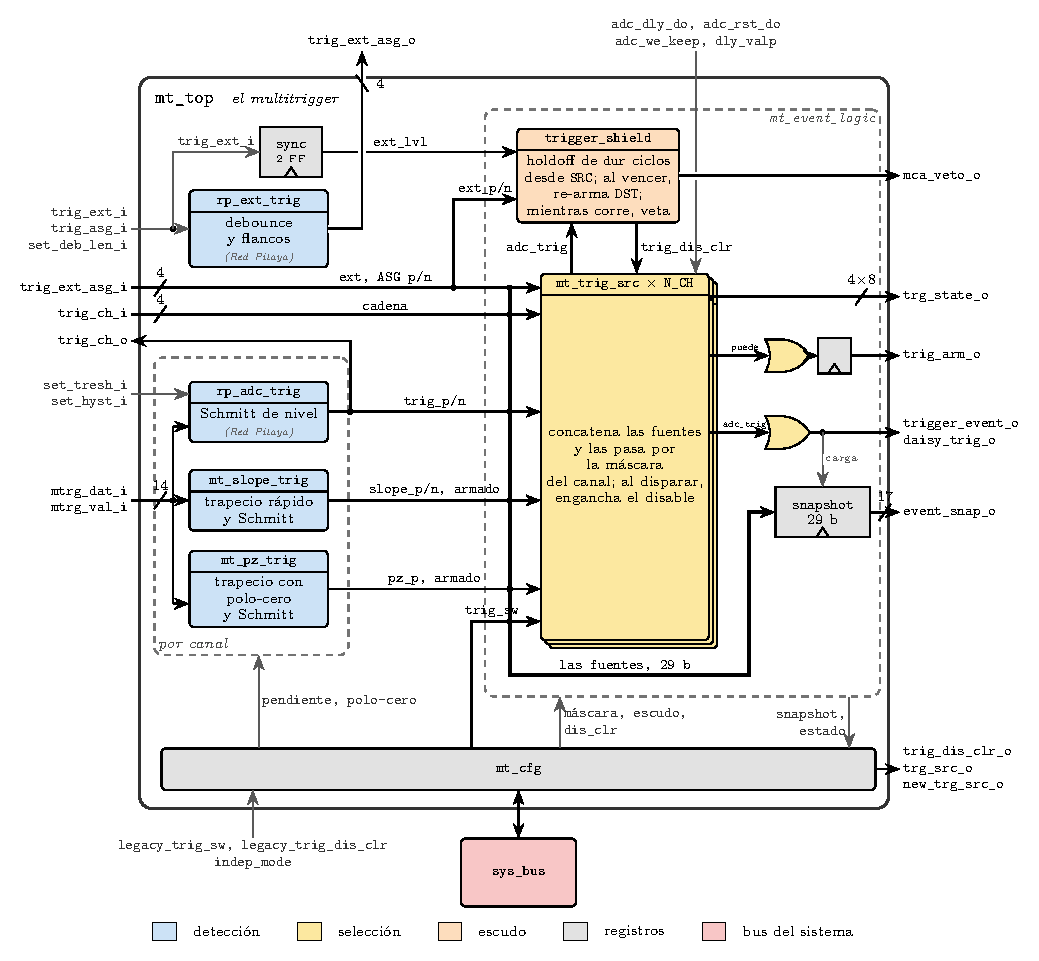
\includegraphics{cap3_panorama_mt}
\caption[Vista general del multitrigger]{%
Vista general del funcionamiento del módulo multitrigger.\label{f:mt-panorama}}
\end{figure}

\begin{table}[H]
\centering
\caption[Submódulos del multitrigger]{%
Submódulos del multitrigger.\label{t:mt-submodulos}}
\footnotesize
\setlength{\tabcolsep}{3pt}
\newcolumntype{Y}{>{\raggedright\arraybackslash}X}
\begin{tabularx}{\textwidth}{|>{\raggedright\arraybackslash}p{0.17\textwidth}|>{\raggedright\arraybackslash}p{0.18\textwidth}|Y|Y|}
\hline
\encabezado \textbf{Submódulo} & \textbf{Función} & \textbf{Entra / sale}
  & \textbf{Decisión de diseño} \\ \hline
\codigo{rp\_adc\_trig} & disparo por nivel, uno por canal
  & muestra $\rightarrow$ flancos \codigo{p}/\codigo{n}
  & el original de Red Pitaya~\cite{RedPitayaFPGA}, sin cambios \\ \hline
\codigo{rp\_ext\_trig} & entrada externa (DIO0\_P)
  & línea externa $\rightarrow$ flancos \codigo{p}/\codigo{n}
  & el original de Red Pitaya; el nivel se sincroniza aparte, para el veto
  \\ \hline
\codigo{mt\_slope\_trig} & disparo por pendiente, uno por canal
  & muestra $\rightarrow$ pulsos \codigo{p}/\codigo{n} y su re-armado
  & una derivada suavizada: el umbral no se mueve con la línea de base \\ \hline
\codigo{mt\_pz\_trig} & disparo por polo-cero, uno por canal
  & muestra $\rightarrow$ pulso y su re-armado
  & el trapecio del MCA, corto: no queda ciego en la cola de un pulso grande
  \\ \hline
\codigo{mt\_trig\_src} & selección de las fuentes de un canal
  & 29 fuentes $\rightarrow$ disparo del canal
  & máscara OR en lugar de un selector; enganche \codigo{adc\_trg\_dis} \\ \hline
\codigo{trigger\_shield} & escudo: \emph{holdoff} y veto
  & disparos y entrada externa $\rightarrow$ \emph{clear} por canal, veto al MCA
  & fuentes y destinos independientes, un solo contador \\ \hline
\codigo{mt\_event\_logic} & une los canales, el escudo y las salidas
  & disparos por canal $\rightarrow$ \codigo{trigger\_event},
    \codigo{trig\_arm}, \emph{snapshot}
  & no tiene lógica de disparo propia: es la topología \\ \hline
\codigo{mt\_cfg} & registros
  & bus del sistema $\rightarrow$ máscaras, escudo, umbrales
  & separado del bus del osciloscopio \\ \hline
\end{tabularx}
\end{table}

Las decisiones de diseño de los submódulos con lógica propia se presentan en la
Sec.~\ref{S:ap-mt-submodulos}. Los puertos y registros de todos están en sus
hojas de datos, en el repositorio.

\subsection{Función de \emph{timestamping}}
\label{S:mt-timestamping}

En el mismo ciclo de reloj del pulso de evento se captura el valor de un contador interno de la PL, que se mantiene hasta el
siguiente evento y funciona como referencia temporal. Este valor sale del módulo
y lo lee el OSC para hacer el \emph{timestamping} de los eventos medidos.

\subsection{Tiempo de relanzamiento}
\label{S:mt-relanzamiento}

Este se refiere al tiempo muerto propio del módulo~\cite{Knoll2010,Muller1973}.
Después de cada disparo, una fuente con histéresis~\cite{Schmitt1938} no puede
volver a disparar hasta re-armarse. Un pulso que llega en ese lapso no genera
flanco y el MCA no lo ve, así que no hay nada que contar. Lo único que se puede
medir es \textbf{cuánto tiempo estuvo desarmado el disparo}, y para eso el MT
expone el estado de re-armado de sus fuentes.

\subsubsection{Señal de re-armado de cada fuente}

Algunas fuentes exponen su señal de re-armado $a_i$, que vale 1 cuando la fuente
puede volver a disparar: los disparos por pendiente (\codigo{mt\_slope\_trig}) y
por polo-cero (\codigo{mt\_pz\_trig}). Las que no la tienen se consideran
siempre armadas, $a_i = 1$: las fuentes sin re-armado propio (manual, externa,
ASG y cadena) y el disparo por nivel (\codigo{rp\_adc\_trig}), que es el
original de Red Pitaya y no expone su estado.

\subsubsection{Relanzamiento del sistema con la OR}

Con la OR, el sistema dispara si dispara cualquiera de las fuentes habilitadas.
El criterio es entonces: \textbf{el sistema está en relanzamiento cuando ninguna
fuente habilitada puede disparar}, es decir, cuando todas están desarmadas. La
señal \codigo{trig\_arm} vale 1 fuera de ese estado. El criterio sólo usa las
señales de re-armado: quien lo consume no necesita saber qué disparo se utiliza.

\subsubsection{Cuándo mide los pulsos perdidos}

El tiempo de relanzamiento se mide para estimar cuántos pulsos se pierden. Ese
paso supone que, si alguna fuente está armada, el pulso se detecta, y eso sólo
vale si la fuente armada \textbf{reacciona a ese pulso}. La condición es
entonces que \textbf{cada fuente habilitada reaccione a todos los pulsos que se
miden}. Si se cumple, el tiempo de relanzamiento coincide con el tiempo en que
el disparo pierde pulsos: es la intersección de los intervalos desarmados de las
fuentes, ya que un pulso que llega con una fuente desarmada entra por otra que
esté armada.

Si no se cumple, una fuente puede estar armada sin reaccionar al pulso. Por
ejemplo, con el polo-cero de IN1 y el de IN2 habilitados y el MCA midiendo IN1:
después de un pulso en IN1, el polo-cero de IN1 queda desarmado, pero el de IN2
sigue armado porque no le llegó nada. \codigo{trig\_arm} vale 1, y un pulso que
llegue a IN1 en ese lapso se pierde contado como \emph{livetime}. Lo mismo pasa con dos
fuentes sobre la misma señal y umbrales distintos: con la de umbral bajo
desarmada, un pulso que no alcanza el umbral alto se pierde. En esos casos
$\mathtt{t\_rearm}$ es una cota inferior. También lo es con las fuentes que no
exponen su estado (nivel, externa), que cuentan como siempre armadas.

% Bibliografía de este capítulo. Va al final del archivo, siempre.
\bibliografiacapitulo

%%% Local Variables:
%%% mode: latex
%%% TeX-master: "template"
%%% End:
